
\chapter{Conclusions and perspectives}
\label{chap:5}

In Chapter 1 we discussed the general state of the art and background for the fields studied in this thesis.
The history and international R\&D projects for Sodium-cooled Fast Reactors (SFR) were briefly reviewed.
The required conditions for acoustic measurement systems for SFRs were then explained.
There are several factors that may decrease the quality of acoustic measurements in a SFR.
For this thesis, we selected the medium heterogeneity as main target among these factors.
The recent studies on thermo-hydraulic state in the core of SFRs were also summarized.
Then, former studies on wave propagation in heterogeneous media, including liquid sodium, were reviewed.
We also discussed former studies on simulation methods for fluctuating media for SFRs.
It was mentioned that the Spectral Element Method (SEM) can be applied as a numerical simulation method
to calculate wave propagation not only in heterogeneous acoustic media but also in elastic media, handling reflection and transmission at acoustic-elastic boundaries accurately.
In this thesis, this will lead to the first-ever application of the SEM for simulation of wave propagation in the cooling medium of SFRs.

In Chapter 2, the derivation of the propagation equations for acoustic and elastic waves in heterogeneous and/or moving media were recalled.
Then, we also briefly summarized several classical numerical methods for wave propagation simulation, including the SEM and Finite-Difference Time-Domain (FDTD) methods.
The numerical code SPECFEM was introduced, which we use to perform the SEM calculations in this thesis; it is an open-source software package with great efficiency,
optimized for high-performance computing, in particular on large computers and on supercomputing centers.

In Chapter 3, we carried out studies for 2D wave propagation simulations in heterogeneous media.
We summarized an experiment called UPSILON, which uses silicon oil as the propagation medium.
This experiment was done by a previous Ph.D. student.
Using the configuration of UPSILON, we carried out a comparison study between the SEM and some FDTD methods.
The result showed the numerical advantage and efficiency of the SEM for our application.
We then applied the SEM to a simplified upper-core region, i.e., the sodium outlet and its surrounding region,
and analyzed the possible amount of acoustic fluctuation for thermometry installed in such a simplified upper-core region of a SFR.
We applied a 2D Gaussian random field technique to represent the medium fluctuations in this part of the study.
We demonstrated that a \num{1}\% change in temperature can be detected by variations in time of flight measured by an ultrasonic transducer.

In Chapter 4, 4D simulations, i.e. spatially 3D with multiple time steps of the medium state, were carried out using an experimental configuration called PLAJEST.
An important result was obtained: we demonstrated that ultrasonic measurements could follow thermo-hydraulic fluctuations with high sensitivity.
We defined a new measurement index called CTFI to describe the variations in the thermo-hydraulic conditions.
We demonstrated a correlation between the second derivative of this index and the second derivative of several ultrasonic measurements,
including time of flight, which would be the easiest to use in practice in a true production setup.
We also showed that frequency variations could be detected using ultrasounds.

\noindent
\underline{Several perspectives for future work can be proposed to further develop the results of this work:}

\subsection*{Schlieren visualization of acoustic waves in a heterogeneous medium}

A first interesting one is to develop comparisons between simulations and experiments to validate all numerical developments with real data.
The experiment UPSILON (see Chapter \ref{chap:3}) may be upgraded to propose a 3D validation by acquiring 3D experimental data.
During this PhD work we began to develop an UPSILON II experiment by using an array of transducer.
Figure \ref{fig:upsilon_vis} shows the results that we obtained using Schlieren observations.
These results confirm those obtained by Massacret and are in accordance with the simulations performed with SPECFEM.
The next step would be to develop 3D acquisition with an array of transducers.
This experiment could also be used to create benchmarks to compare SPECFEM results to those obtained with other software packages dedicated to ultrasonic NDT simulation,
such as CIVA, and to real data.
In that case, introducing the precise modeling of an array of transducers in SPECFEM could also be an interesting new development for this code.
An array of transducers may also be a more suitable device to follow in a precise way thermo-hydraulic conditions such as the deviation of the spot (maximum of the wave),
as in Figure \ref{fig:impactpoint}.

\begin{figure}[htbp]
    \centerline{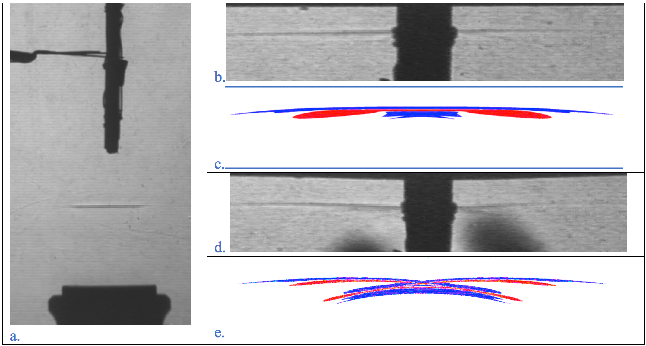
\includegraphics[width=17.0cm]{upsilon_vis.pdf}}
    \slantedcaption{Schlieren visualization of wave distortion due to thermal gradient, and corresponding simulations with SPECFEM.
    a.  Wave propagation between the transducer (bottom) and the electric wires (up).
    b.  Wave front without a temperature gradient.
    c.  Wave front simulation using SPECFEM2D.
    d.  Wave front with a temperature gradient.
    e.  Wave front simulation including a thermal gradient in the medium (see Chapter \ref{chap:3}).}
    \label{fig:upsilon_vis}
\end{figure}

\clearpage
\subsection*{3D numerical simulations for a complex geometry}

A second perspective is to use the 3D potential of SPECFEM to perform simulations for realistic, and thus complex, geometries of targets.
As an example, in Figure~\ref{fig:comp_mesh}  we generated (using SOLIDWORKS) a geometry resembling the sodium outlet tube of the Phenix reactor.
 Part (c) of the figure shows the model meshed with tetrahedral elements, and (b) and (d) are the model meshed with hexahedral elements.
 Part (b) represents the whole model, i.e. the acoustic (liquid sodium) part and the elastic (steel) part.
 The elements in red in Part (e) are those whose Jacobian values are negative, i.e. those for which the mesh created is not usable because it is too distorted.
 Such meshing failure can occur for instance when a hexahedra-meshed geometry contains shapes such as holes or concavities.
 Most finite-element methods used in industry thus resort to tetrahedral elements because they almost never lead to such elements with a negative Jacobian (but quality degradation by sliver elements may happen) and mesh generation is done almost automatically without manual intervention by a skilled computer-aided engineer (CAE),
 which is almost always necessary for hexahedral-meshed models in the case of its having complex geometry.
However, hexahedra-based techniques (such as the SEM, among others) lead to tensorized basis functions and thus to very significantly faster calculations.
 At the moment SPECFEM3D supports only hexahedral elements, in order to take advantage of such tensorized basis functions, and thus a drastically reduced number of nested
loops in the calculations.
 In addition, as mentioned above, the SEM has the advantage of the high accuracy of the calculations because of spectral-like convergence properties \parencite{KoMaTrTaWi01}.
In future work it could thus be worth investigating the use of triangular elements in 2D or tetrahedral elements in 3D in addition to hexahedra,
following for instance the ideas of \cite{Dub93}, \cite{KoMaTrTaWi01} and \cite{PaRa04} in 2D and their extension to 3D by \cite{ShKarn95}.
Note however that to mix tetrahedra with hexahedra, for geometrical reasons, due to the need to have a geometrically-conforming mesh, one would also need to introduce pyramidal
elements for the transition region.
Note also that the geometry of the ASTRID reactor sub-assembly heads is expected to be simpler than those of Phenix,
or with complex geometry only far from the top of the heads, and thus such meshing difficulties based on hexahedra only may also not occur in practice.

\subsection*{Calculation methods for a moving medium and for temporal changes of the medium heterogeneity}

In this thesis we have used the so-called `frozen fluid' hypothesis, i.e. the flow velocity field did not have an effect on wave propagation
and the state of the heterogeneous medium did not change during a given calculation. This resorted to using snapshots taken at different times
in such a moving medium, and performing numerical simulations for each of them (independently), considering each of them as static.
This assumption was applied following the result of \cite{Massacret2012Simplifiedmodelingof}, who said that the effect of the flow velocity temporal gradient is less important
than the effects coming from temperature gradients, at least for his simplified upper-core region model
(the effects coming from the flow velocity temporal gradient was about five times smaller than that coming from the temperature gradient).
However that study also mentions that it is not clear if the `frozen fluid' hypothesis is applicable to more complex gradient fields
(in the study of \cite{Massacret2012Simplifiedmodelingof}, a gradient field having a simple cylindrical shape was used for their ray-tracing calculation).
Also, when the propagation distance is very long, the gradient field may change during the propagation and thus the `frozen fluid' approximation may not be applicable any more.

\noindent
At the end of this thesis, we still have no new knowledge about how the amount of acoustic fluctuation will be changed
by the influence of temporal changes of the medium heterogeneity, as the general hypothesis of frozen fluid seems to be valid even for the PLAJEST experiment.
Thus, in order to study the effect of such a transient medium, further studies will be necessary. For instance, acoustic wave propagation simulations
that take into account the flow gradient field, with a realistic heterogeneous medium coming for instance from the PLAJEST data, could be performed.
However we currently have no SEM code that may take into account such a moving medium. Support for moving media, following for instance the initial numerical work
of \cite{KaDu08} for a flow with constant and uniform velocity, should be added.
However, this may be technically complex because in such a case Equation \ref{eq:1_43} needs to be used,
but this equation has a third-order temporal derivative term, which would imply changing the whole time scheme that is used in the SPECFEM code as well
as in other classical SEM software packages.
One possible option to consider would be to calculate this third-order derivative using some approximation; \cite{Ashyralyev2007Anoteon} for instance
proposed an approximation using a Taylor decomposition.
Another option would be to implement a new time-marching scheme, suitable for third-order time derivatives.

\begin{figure}[htbp]
    \centerline{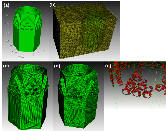
\includegraphics[width=17.0cm]{comp_mesh.pdf}}
    \slantedcaption{
    Examples of 3D meshing of a realistic geometry.
    (a) is an example of 3D relatively complex geometry resembling the sodium outlet of Phenix, created using SOLIDWORKS.
    (b) shows the entire geometry meshed with hexahedral elements.
    (c) is the meshed tube with tetrahedral elements.
    (d) is the same geometry but meshed with hexahedral elements.
    (e) shows the hexahedral elements that have a negative Jacobian and are thus unsuitable for numerical calculation.}
    \label{fig:comp_mesh}
\end{figure}

\clearpage
\noindent
Our work shows that acoustic measurements could help in thermal hydraulic mock-up studies, as a complement to thermal measurements.
Ultrasonic temperature measurements and SONAR studies could be improved by considering realistic temperature fluctuations at the outlet of subassembly heads,
provided that time histories are available in the same way as in the PLAJEST simulation using a LES turbulent model.
The SEM could be a powerful tool to study the effects of thermal hydraulics on acoustic wave propagation and take into account the elastic interaction of the waves with the 3D targets.
We also think that the use of supercomputers to perform such expensive simulations, as has been demonstrated in this work,
will become even more useful in the near future because of the massive amount of data (`big data') that has to be handled nowadays.
Such tools should be able to provide new insights to enrich future discussions between thermo-hydraulicians and acousticians.

